\section*{Analysis}
\label{sec:analysis}

Figure~\ref{fig:benchmarks} shows the output of the benchmarks run~\footnote{We would like to know how we can present these results better}.
The results show the benchmarks being run on 4 different hardware.
The hardware specification is shown in Table~\ref{table:hardware}.


\begin{table}[h]\small
\centering
\begin{tabular}{ | l | c | c | c |}
    \hline 
    Name & CPU & GPU & Memory \\ \hline
    GNex & ARMv7 2core 1200 Mhz & PowerVR-SGX 540 & 694Mb \\ \hline
    Nex5 & Snapdragon S4 Pro 1.5GHz & Adreno320 400MHz & 2Gb} \\ \hline
    Nex7 & Snapdragon 800 2.26GHz & Adreno330 450MHz & 2Gb} \\ \hline
    T900 & Quad-core 1.9 GHz Cortex-A15 & Mali-T628 MP6 & 3Gb} \\ \hline
    \hline
\end{tabular}
\caption{The hardware specifications of the devices we ran the benchmarks on.}
\label{table:hardware}
\end{table}

\begin{figure}%
    \centering
    \subfloat[VectorAdd]{{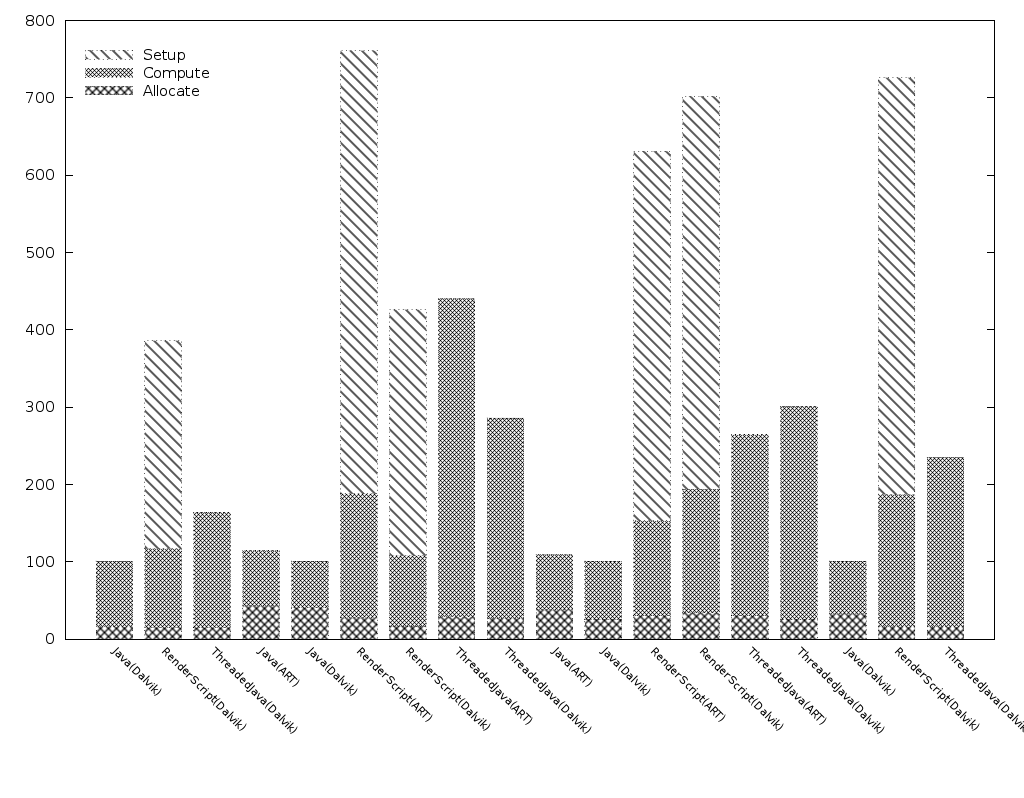
\includegraphics[width=0.5\linewidth]{vecadd} }}~
    \subfloat[SGEMM]{{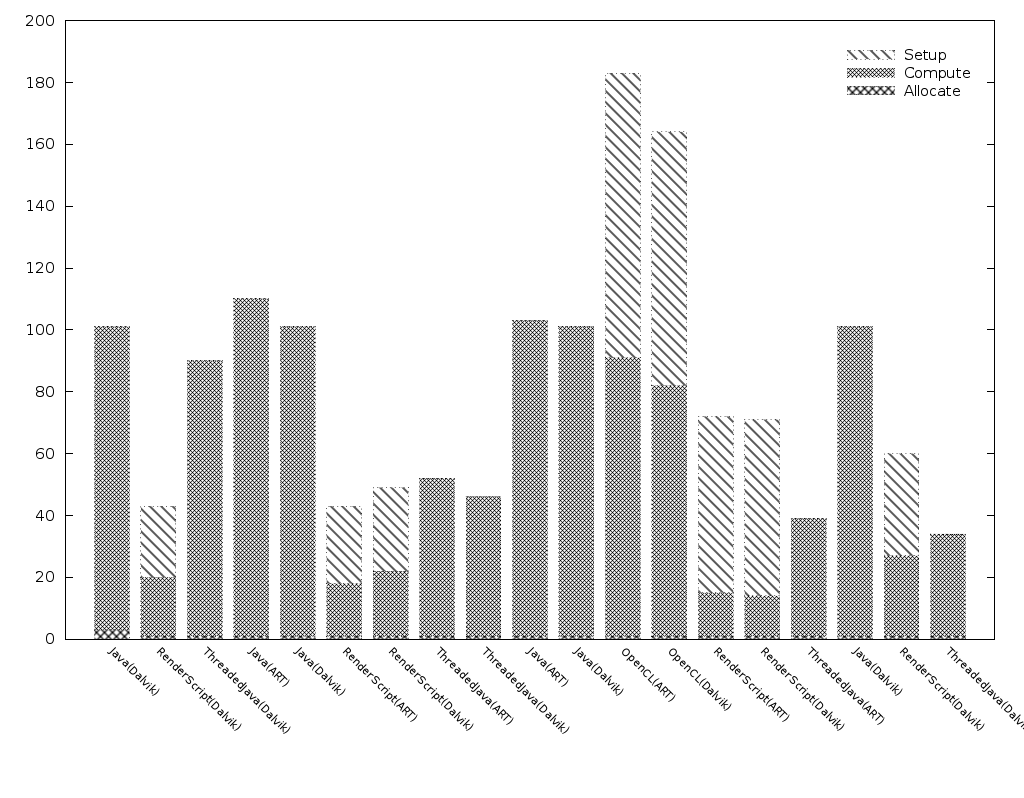
\includegraphics[width=0.5\linewidth]{sgemm} }}\\
    \subfloat[MRI-Q]{{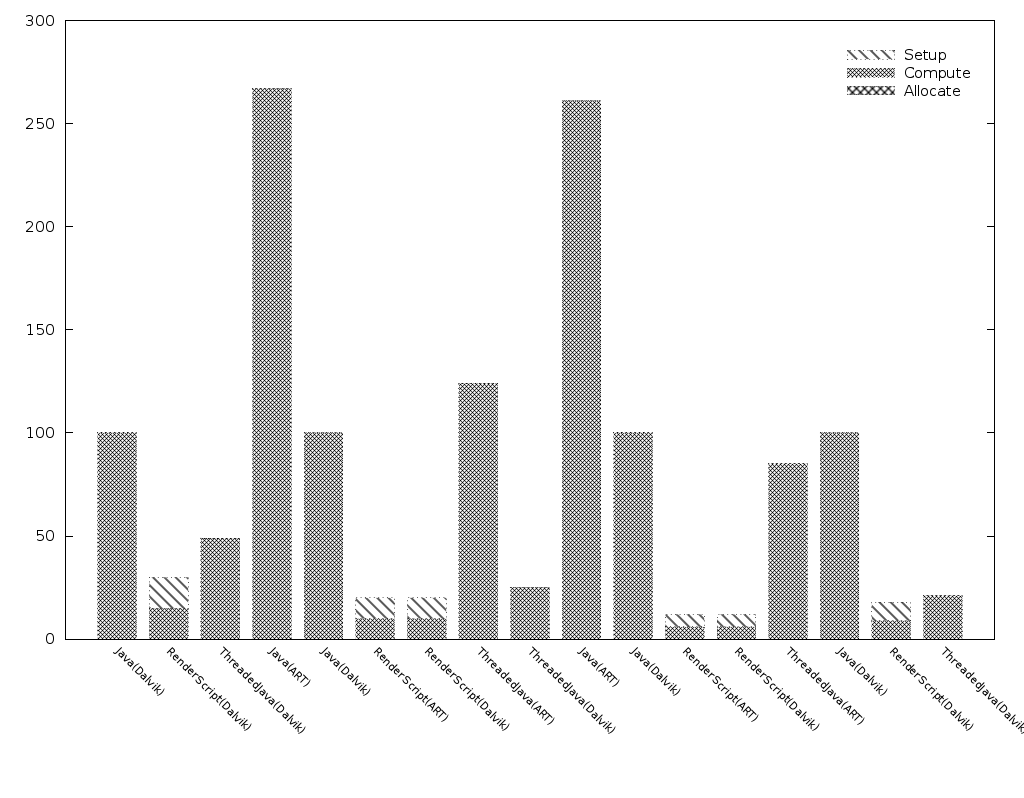
\includegraphics[width=0.5\linewidth]{mriq} }}~
    \subfloat[TPACF]{{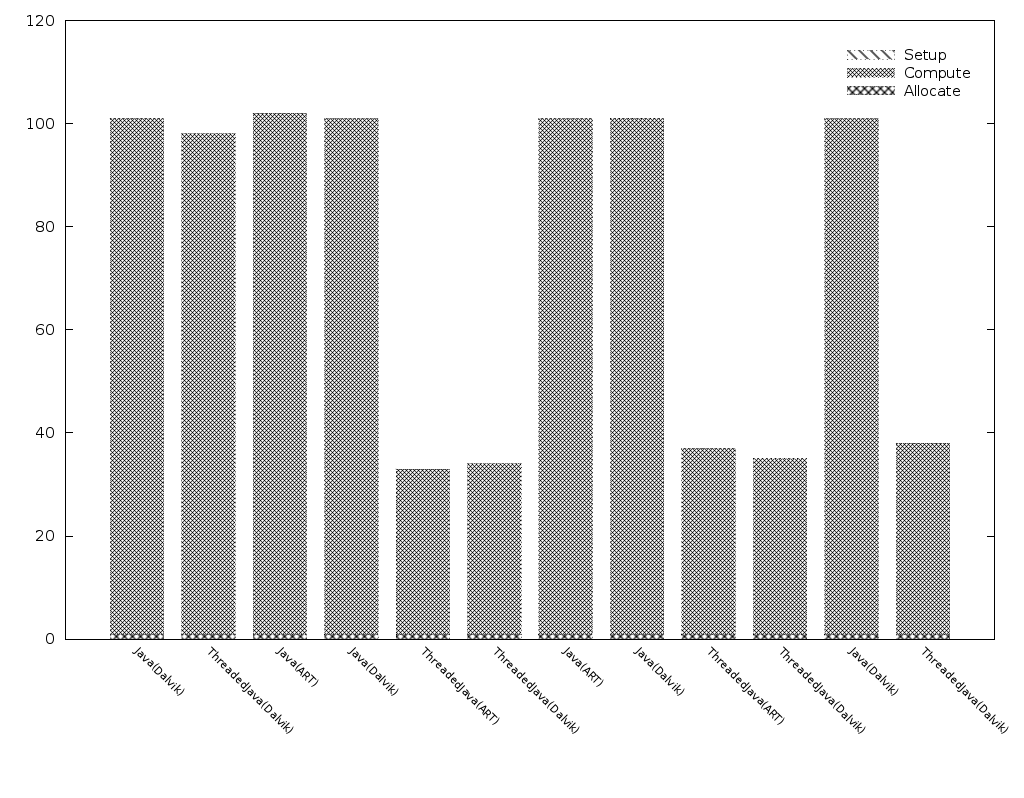
\includegraphics[width=0.5\linewidth]{tpacf} }}\\
    \subfloat[Stencil]{{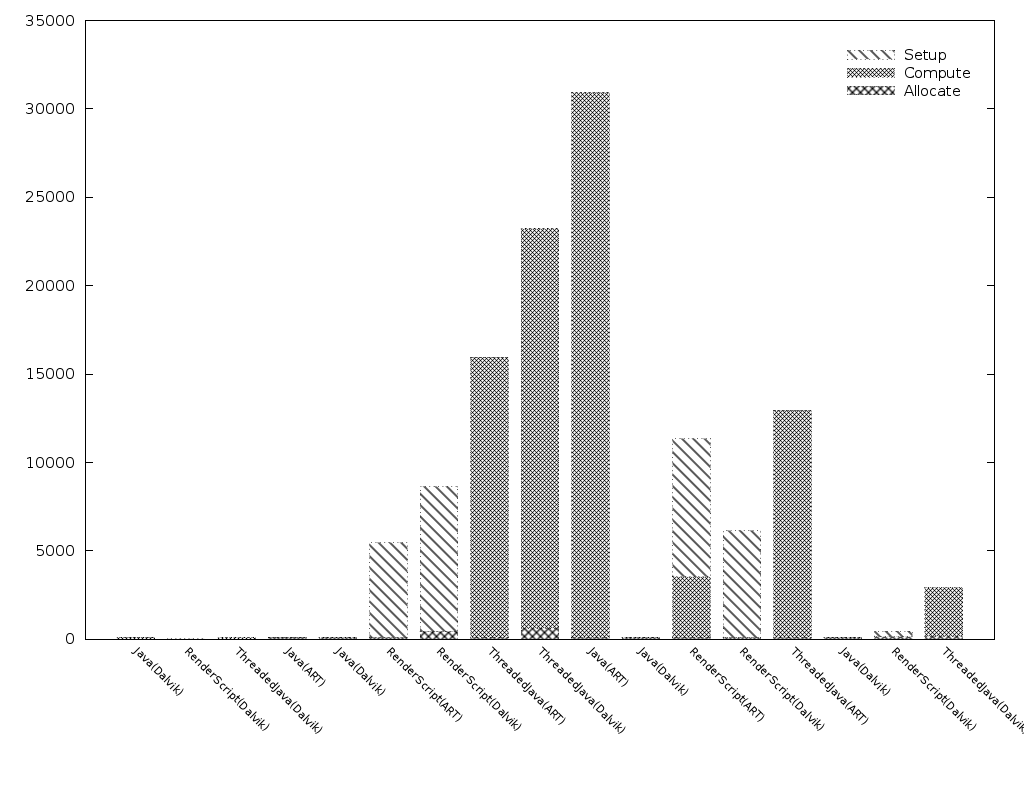
\includegraphics[width=0.5\linewidth]{stencil} }}~
    \subfloat[Histogram]{{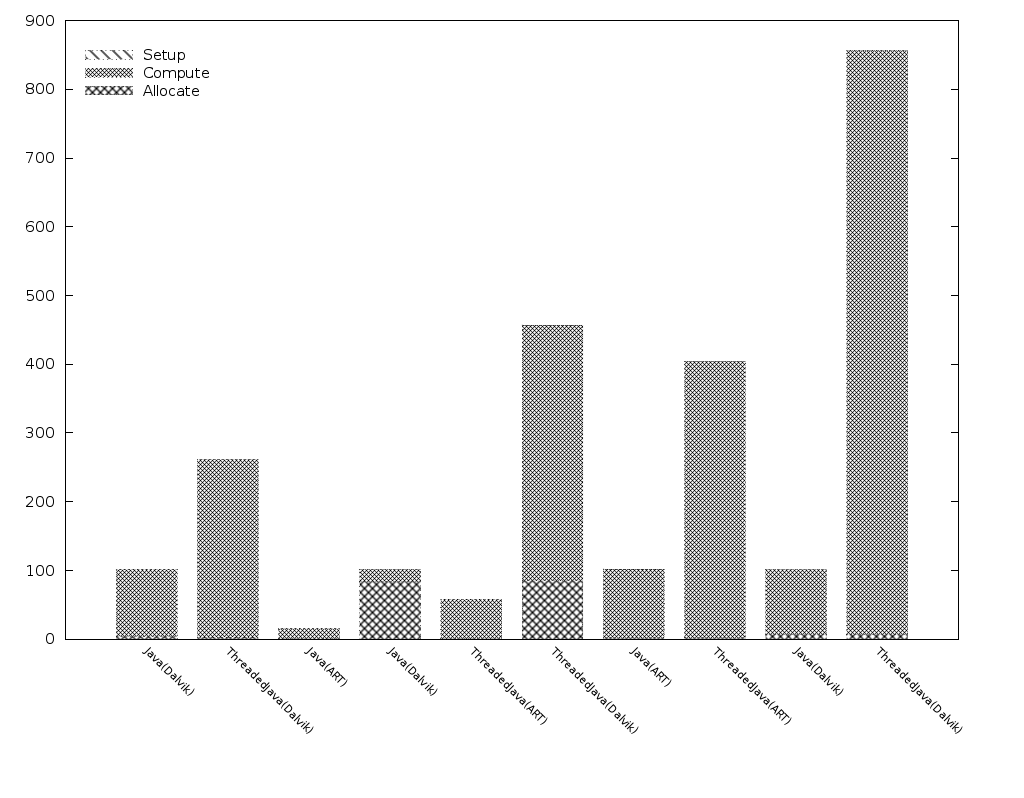
\includegraphics[width=0.5\linewidth]{histogram} }}%
    \caption{Benchmark results: yellow corresponds to runs being performed on GNex, Red on the Nex5, Green on the Nex7, and Blue on the T900.}%
    \label{fig:benchmarks}%
\end{figure}


